% DO NOT COMPILE THIS FILE DIRECTLY!
% This is included by the other .tex files.

\begin{frame}[t,plain]
\titlepage
\end{frame}

\begin{frame}
    \frametitle{Content of the presentation}
    \begin{itemize}
        \item Data sharing in MISP
        \item Data models for the Data layer
        \item Data models for the Context layer
    \end{itemize}
\end{frame}

\begin{frame}
    \frametitle{Layers of data model}
     \begin{itemize}
            \item Data layer
            \begin{itemize}
                \item The raw data itself as well as element to link them together
                \item Indicators, Observables and means to contextually link them
                \item MISP terminology: Event, Attributes, misp-objects, ...
            \end{itemize}
            \vspace{1em}
            \item Context layer
            \begin{itemize}
                \item As important as the data layer, allow triage, false-positive management, risk-assessment and prioritisation
                \item Latches on the data layer, usually referencing threat intelligence, concepts, knowledge base and vocabularies
                \item Tags, Taxonomies, Galaxies, ...
            \end{itemize}
    \end{itemize}
\end{frame}

\section{Data sharing in MISP}
\begin{frame}
    \frametitle{Sharing in MISP: Distribution}
    MISP offers granulars distribution settings:
    \begin{itemize}
        \item \texttt{Organisation only}
        \item \texttt{This community}
        \item \texttt{Connected communities}
        \item \texttt{All communities}
        \item Distribution lists - aka \texttt{\bf Sharing groups}
    \end{itemize}
    \begin{center}
    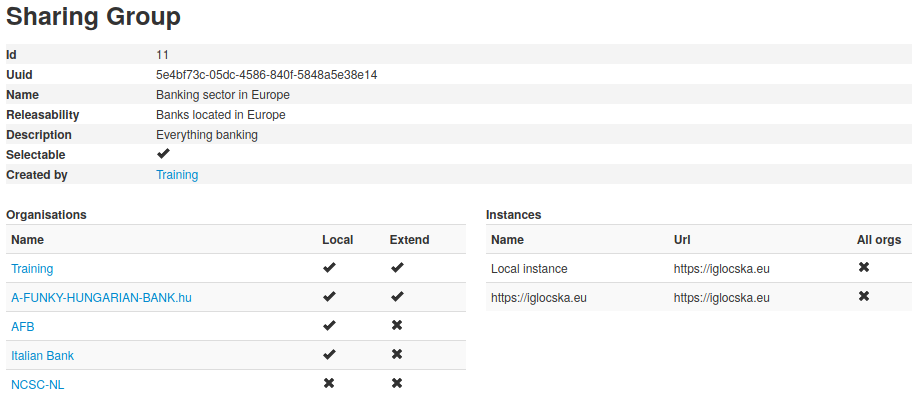
\includegraphics[scale=0.2]{screenshots/sg-example.png}
    \end{center}

    At multiple levels: {\bf Events}, {\bf Attributes}, {\bf Objects} (and their {\bf Attributes}) and {\bf Galaxy-clusters}
\end{frame}

\begin{frame}
\frametitle{Sharing in MISP: Distribution}
    \begin{center}
        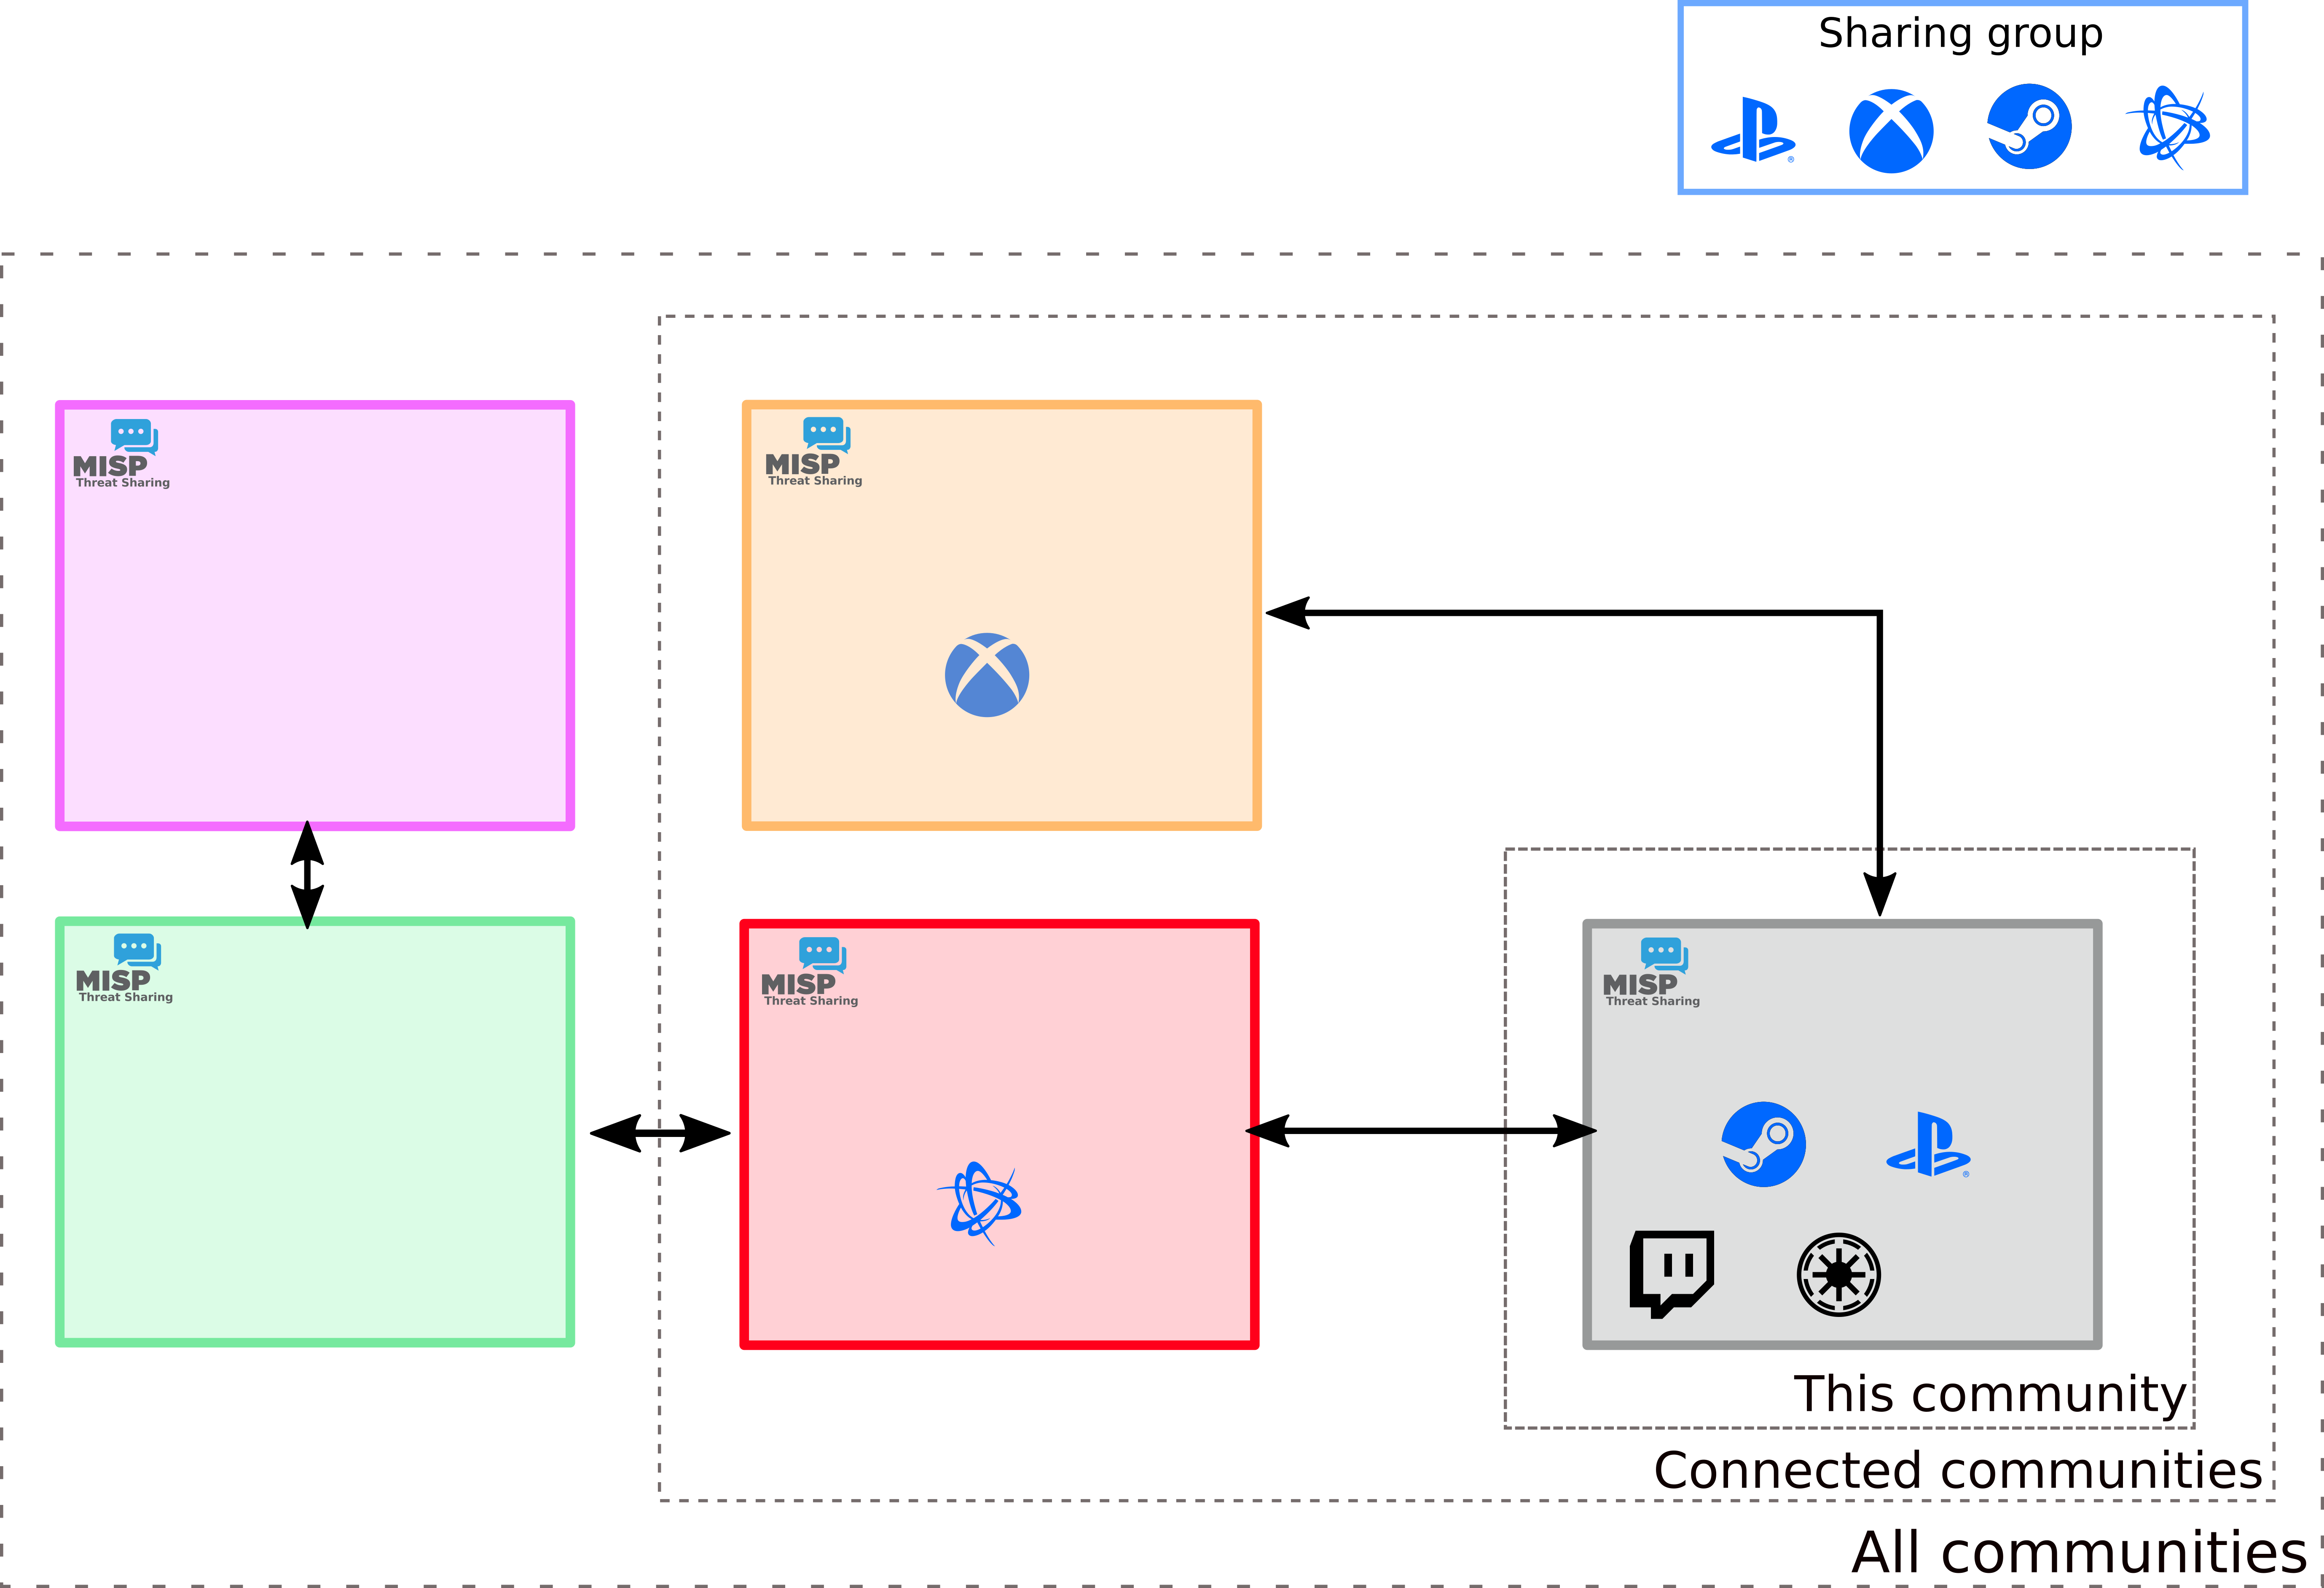
\includegraphics[width=1.0\linewidth]{screenshots/misp-distribution.png}
    \end{center}
\end{frame}

\section{Data layer}
\begin{frame}
    \frametitle{Data layer: Naming conventions}
     \begin{itemize}
            \item Data layer
            \begin{itemize}
                \item {\bf Events} are encapsulations for contextually linked information
                \item {\bf Attributes} are individual data points, which can be indicators or supporting data.
                \item {\bf Objects} are custom templated Attribute compositions
                \item {\bf Object references} are the relationships between individual building blocks
                \item {\bf Shadow Attributes}/{\bf Proposal} are suggestions made by users to modify an existing {\it attribute}
                \item {\bf Sightings} are a means to convey that a data point has been seen
                \item {\bf Event reports} are supporting materials for analysts to describe {\it events}, {\it processes}, etc
            \end{itemize}
    \end{itemize}
\end{frame}

\begin{frame}[fragile]
    \frametitle{Data layer: Events}
        {\bf Events} are encapsulations for contextually linked information
        \begin{itemize}
            \item[] \textbf{Purpose}: Group datapoints and context together. Acting as an envelop, it allows setting distribution and sharing rules for itself and its children.
            \item[] \textbf{Usecase}: Encode incidents / events / reports / ...
        \end{itemize}
        \begin{center}
            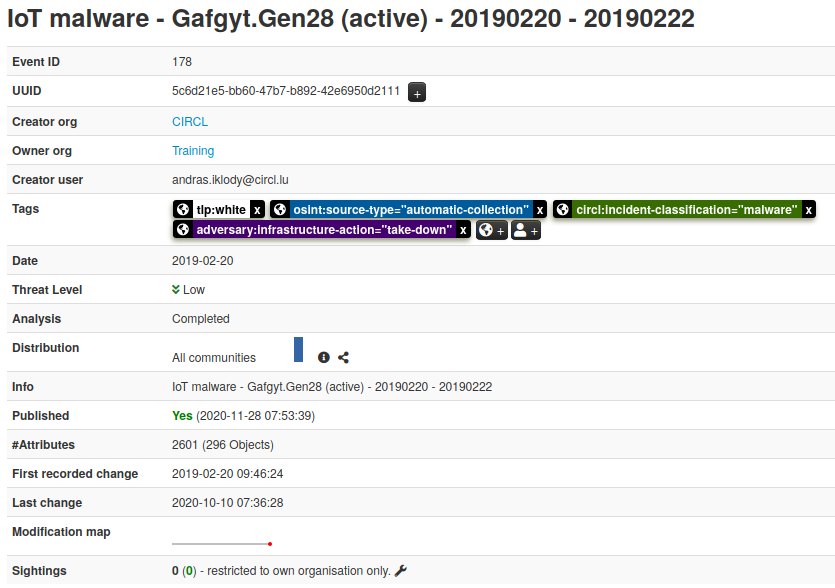
\includegraphics[width=0.7\linewidth]{screenshots/ui-event.png}
        \end{center}
\end{frame}

\begin{frame}
    \frametitle{Data layer: Event building blocks - Base}
        \begin{center}
            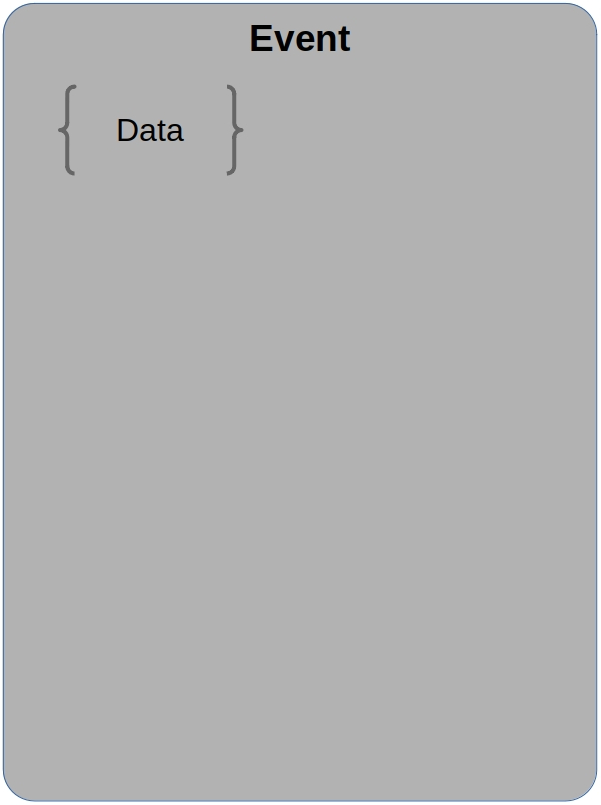
\includegraphics[scale=0.33]{screenshots/event-building-blocks/event.png}
        \end{center}
\end{frame}

\begin{frame}[fragile]
    \frametitle{Data layer: Events}
        \begin{lstlisting}[language=javascript,firstnumber=1]
{
    "date": "2019-02-20",
    "info": "IoT malware - Gafgyt.Gen28 (active)",
    "uuid": "5c6d21e5-bb60-47b7-b892-42e6950d2111",
    "analysis": "2",
    "timestamp": "1602315388",
    "distribution": "3",
    "sharing_group_id": "0",
    "threat_level_id": "3",
    "extends_uuid": "",
    "Attribute": [...],
    "Object": [...],
    "EventReport": [...],
    "Tag": [...],
    "Galaxy": [...]
}
\end{lstlisting}
\end{frame}

\begin{frame}[fragile]
    \frametitle{Data layer: Attributes}
        {\bf Attributes} are individual data points, indicators or supporting data
        \begin{itemize}
            \item[] \textbf{Purpose}: Individual data point. Can be an indicator or supporting data.
            \item[] \textbf{Usecase}: Domain, IP, link, sha1, attachment, ...
        \end{itemize}
        \begin{center}
            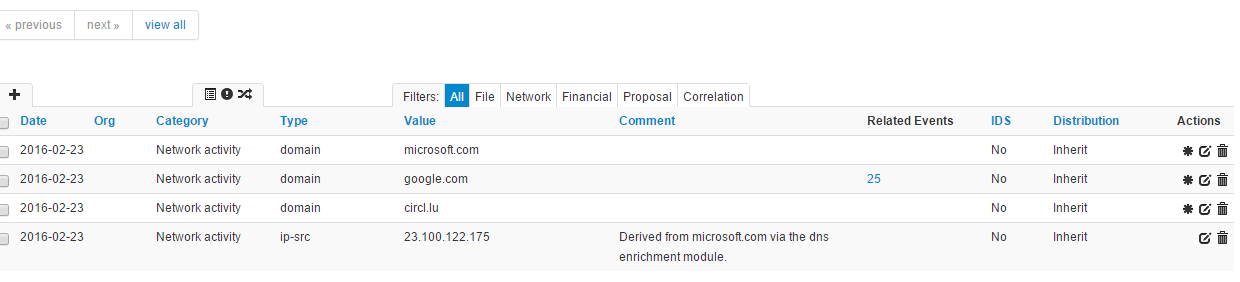
\includegraphics[width=1.0\linewidth]{screenshots/enrichment4.png}
        \end{center}
\end{frame}

\begin{frame}
    \frametitle{Data layer: Event building blocks - Raw data}
        \begin{center}
            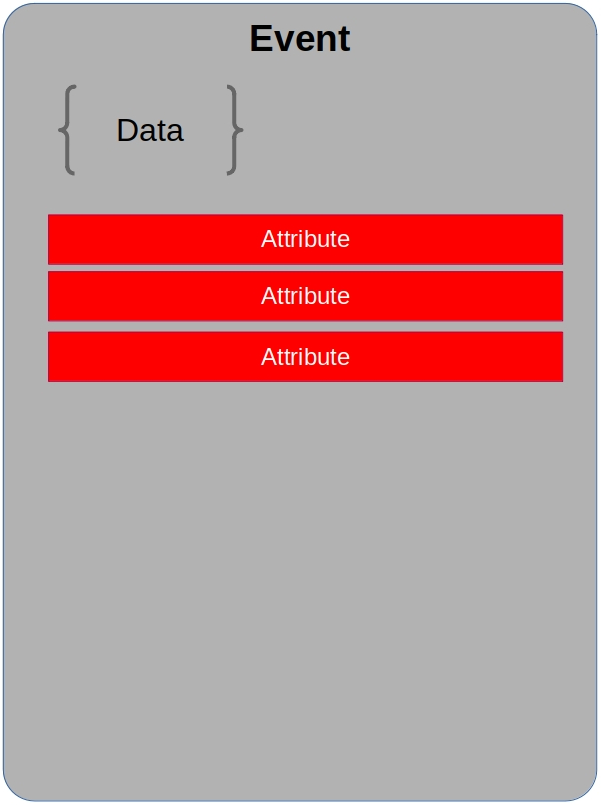
\includegraphics[scale=0.33]{screenshots/event-building-blocks/event-attribute.png}
        \end{center}
\end{frame}

\begin{frame}[fragile]
    \frametitle{Data layer: Attributes}
        \begin{lstlisting}[language=javascript,firstnumber=1]
{
    "type": "url",
    "category": "Network activity",
    "to_ids": true,
    "uuid": "5c6d24bd-d094-4dd6-a1b6-4fa3950d2111",
    "event_id": "178",
    "distribution": "5",
    "sharing_group_id": "0",
    "timestamp": "1550656701",
    "comment": "Delivery point for the malware",
    "object_id": "0",
    "object_relation": null,
    "first_seen": null,
    "last_seen": null,
    "value": "ftp://185.135.80.163/",
    "Tag": [...]
    "Galaxy": [...]
}
\end{lstlisting}
\end{frame}

\begin{frame}
    \frametitle{Data layer: MISP Objects}
        {\bf Objects} are custom templated Attribute compositions
        \begin{itemize}
            \item[] \textbf{Purpose}: Groups Attributes that are intrinsically linked together
            \item[] \textbf{Usecase}: File, person, credit-card, x509, device, ...
        \end{itemize}
        \begin{center}
            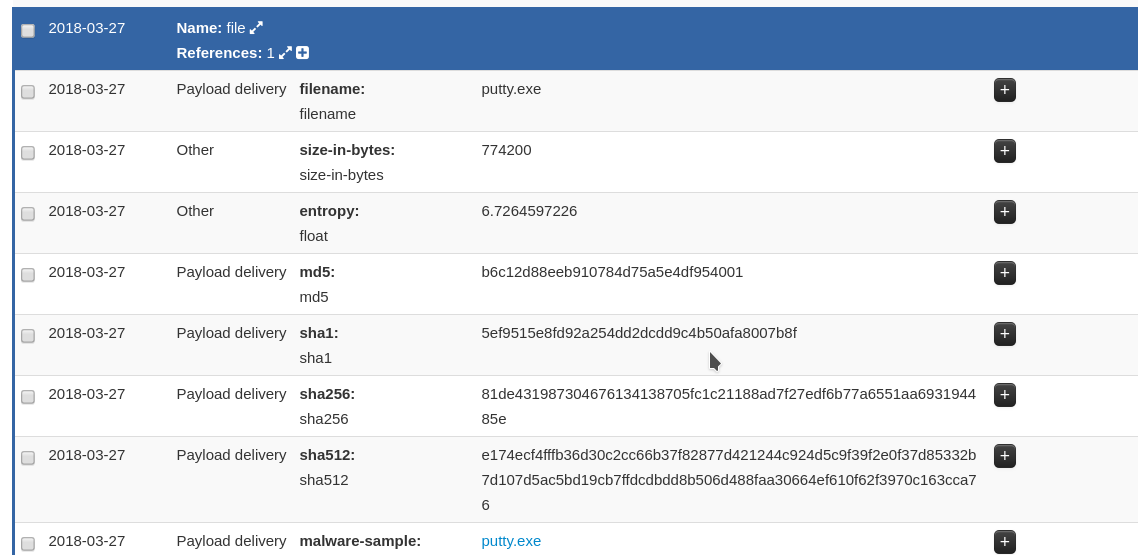
\includegraphics[width=1.0\linewidth]{object.png}
        \end{center}
\end{frame}

\begin{frame}
    \frametitle{Data layer: Event building blocks - Data composition}
        \begin{center}
            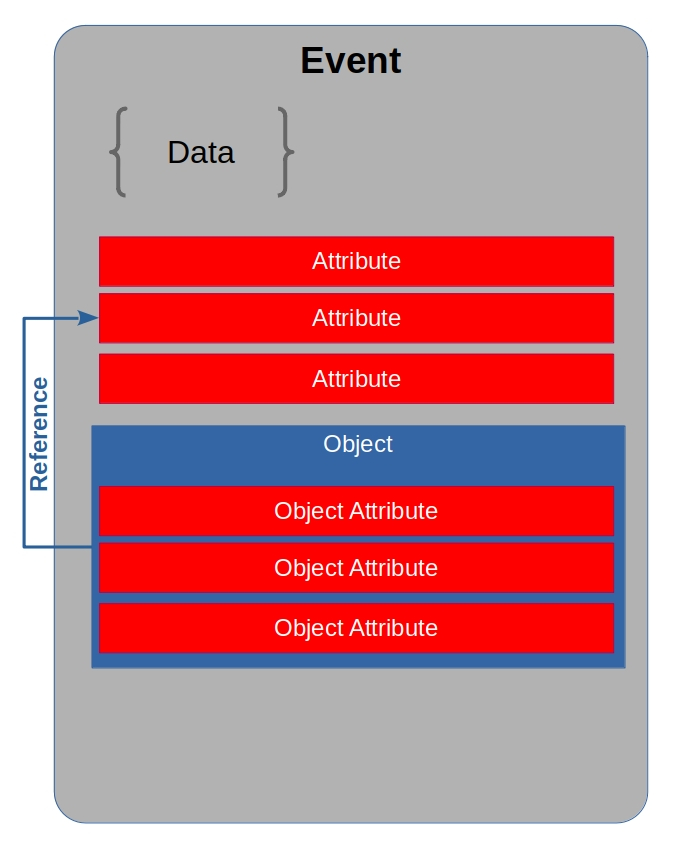
\includegraphics[scale=0.33]{screenshots/event-building-blocks/event-attribute-object.png}
        \end{center}
\end{frame}

\begin{frame}[fragile]
    \frametitle{Data layer: MISP Objects}
        \begin{lstlisting}[language=javascript,firstnumber=1]
{
    "name": "elf-section",
    "meta-category": "file",
    "description": "Object describing a sect...",
    "template_uuid": "ca271f32-1234-4e87-b240-6b6e882de5de",
    "template_version": "4",
    "uuid": "ab5f0c85-5623-424c-bc03-d79841700d74",
    "timestamp": "1550655984",
    "distribution": "5",
    "sharing_group_id": "0",
    "comment": "",
    "first_seen": null,
    "last_seen": null,
    "ObjectReference": [],
    "Attribute": [...]
}
\end{lstlisting}
\end{frame}

\begin{frame}[fragile]
    \frametitle{Data layer: Object references}
    {\bf Object references} are the relationships between individual building blocks
    \begin{itemize}
        \item[] \textbf{Purpose}: Allows to create relationships between entities, thus creating a graph where they are the edges and entities are the nodes.
        \item[] \textbf{Usecase}: Represent behaviours, similarities, affiliation, ...
    \end{itemize}
    \begin{center}
        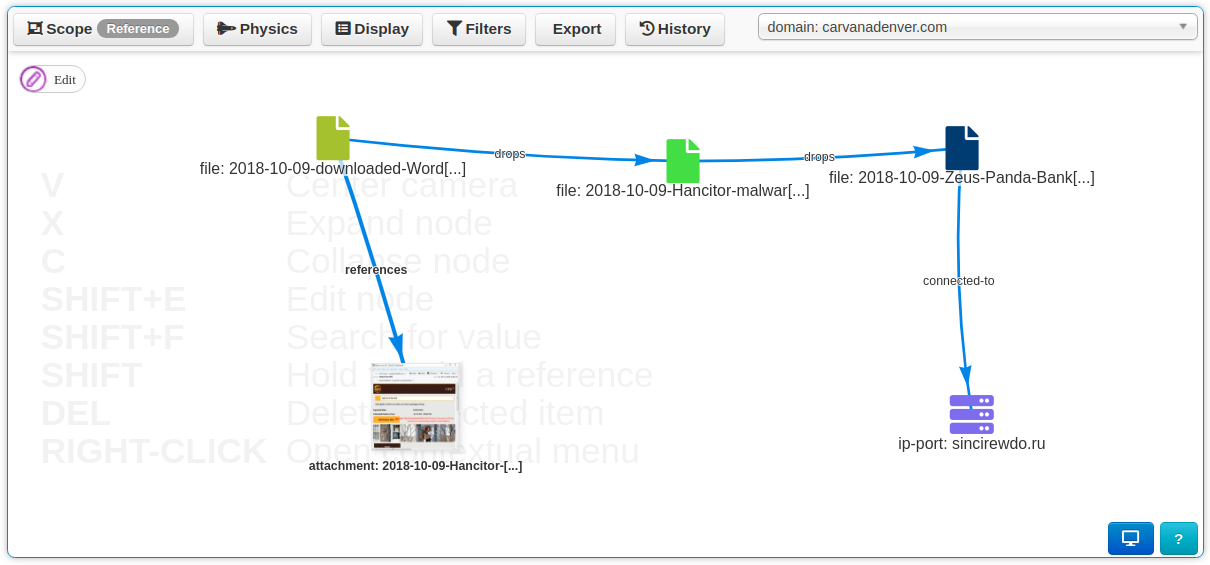
\includegraphics[width=0.9\linewidth]{screenshots/eventgraph.png}
    \end{center}
\end{frame}

\begin{frame}[fragile]
    \frametitle{Data layer: Object references}
    \begin{lstlisting}[language=javascript,firstnumber=1]
{
    "uuid": "5c6d21f9-0384-4bd2-b256-40de950d2111",
    "timestamp": "1602318569",
    "object_id": "1024",
    "source_uuid": "23275e05-c202-460e-aadf-819c417fb326",
    "referenced_uuid": "ab5f0c85-5623-424c-bc03-d79841700d74",
    "referenced_type": "1",
    "relationship_type": "included-in",
    "comment": "Section 0 of ELF"
}
\end{lstlisting}
\end{frame}

\begin{frame}
    \frametitle{Data layer: Event building blocks - Context}
        \begin{center}
            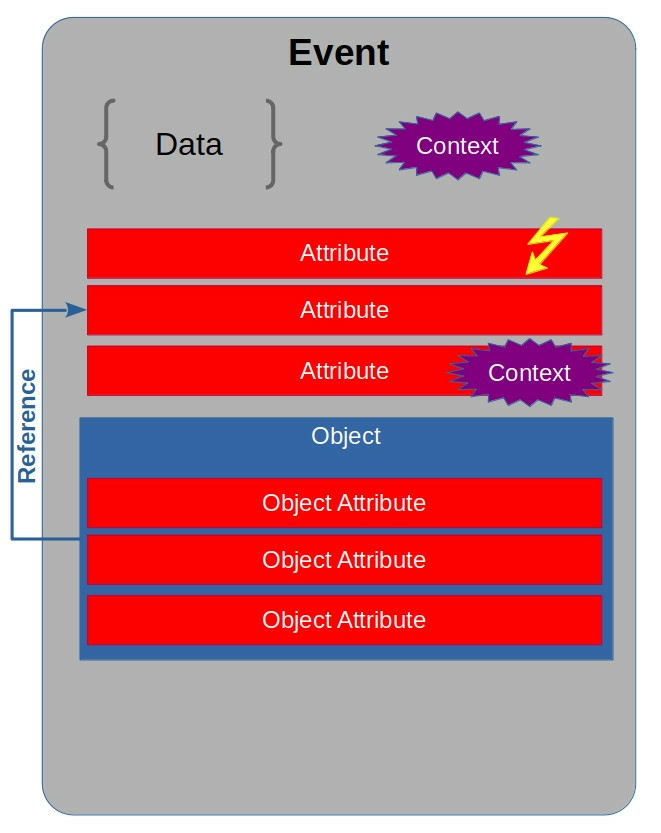
\includegraphics[scale=0.33]{screenshots/event-building-blocks/event-attribute-object-context.png}
        \end{center}
\end{frame}

\begin{frame}[fragile]
    \frametitle{Data layer: Sightings}
    {\bf Sightings} are a means to convey that a data point has been seen
    \begin{itemize}
        \item[] \textbf{Purpose}: Allows to add temporality to the data.
        \item[] \textbf{Usecase}: Record activity or occurence, perform IoC expiration, ...
    \end{itemize}
    \begin{center}
        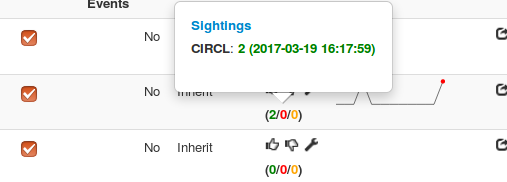
\includegraphics[width=0.7\linewidth]{screenshots/sighting-n.png}
    \end{center}
    \begin{lstlisting}[language=javascript,firstnumber=1]
{
    "org_id": "1",
    "date_sighting": "1573722432",
    "uuid": "5dcd1940-5de8-4462-93dd-12a2a5e38e14",
    "source": "",
    "type": "0",
    "attribute_uuid": "5da97b59-9650-4be2-9443-2194a5e38e14"
}
\end{lstlisting}
\end{frame}

\begin{frame}[fragile]
    \frametitle{Data layer: Event reports}
    {\bf Event reports} are supporting data for analysis to describe {\bf events}, {\bf processes}, ect
    \begin{itemize}
        \item[] \textbf{Purpose}: Supporting data point to describe events or processes
        \item[] \textbf{Usecase}: Encode reports, provide more information about the Event, ...
    \end{itemize}
    \begin{center}
        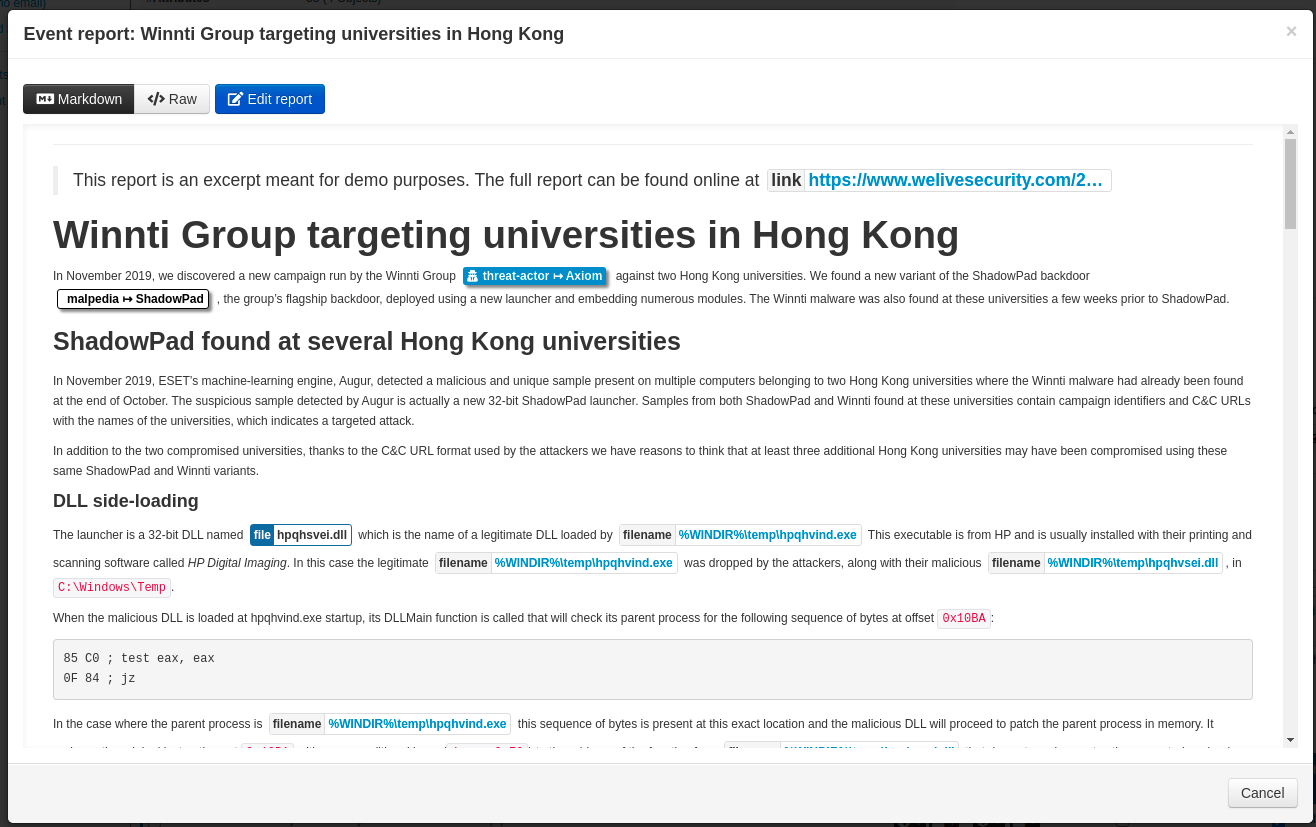
\includegraphics[width=0.7\linewidth]{screenshots/event-report.png}
    \end{center}
\end{frame}

\begin{frame}
    \frametitle{Data layer: Event building blocks - Collaboration \& intelligence}
        \begin{center}
            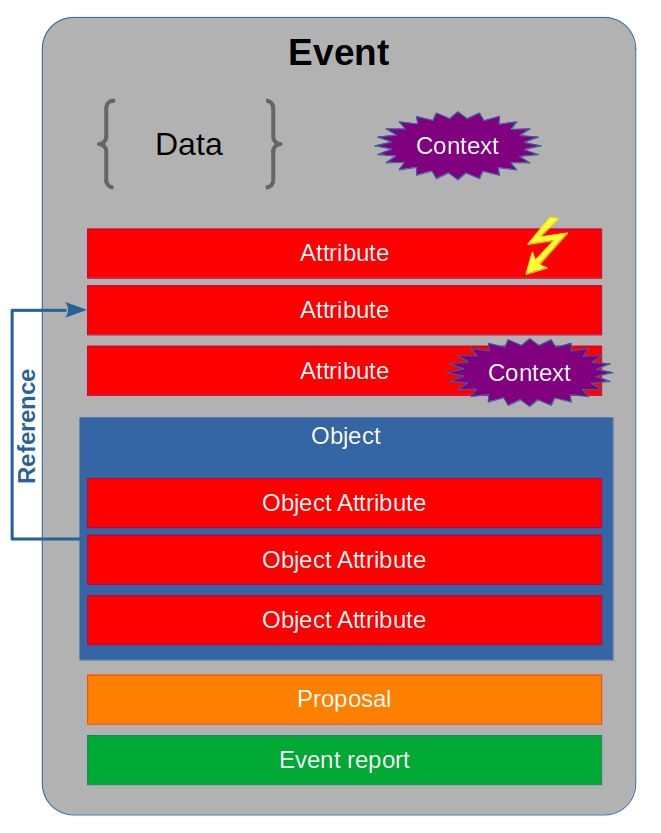
\includegraphics[scale=0.33]{screenshots/event-building-blocks/event-attribute-object-proposal.png}
        \end{center}
\end{frame}

\begin{frame}[fragile]
    \frametitle{Data layer: Event reports}
    \begin{lstlisting}[language=javascript,firstnumber=1]
{
    "uuid": "076e240b-5a76-4a8b-9eab-cfff551993dd",
    "event_id": "2127",
    "name": "Event report (1607362986)",
    "content": "...",
    "distribution": "5",
    "sharing_group_id": "0",
    "timestamp": "1607362986"
}
\end{lstlisting}
\end{frame}

\begin{frame}
    \frametitle{Data layer: Event building blocks - Full}
        \begin{center}
            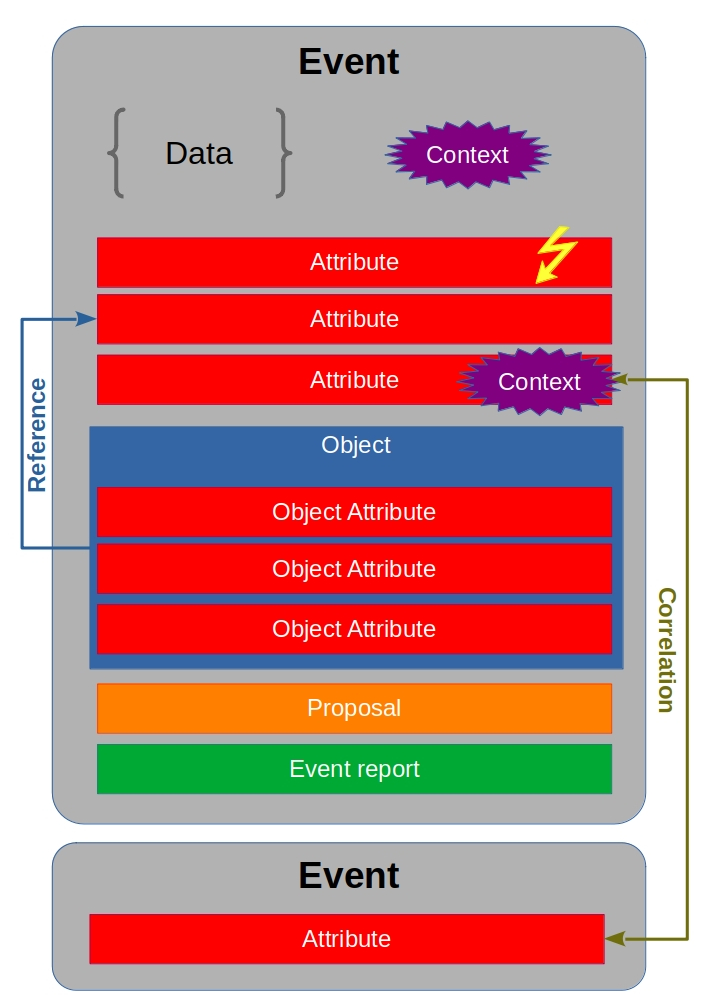
\includegraphics[scale=0.30]{screenshots/event-building-blocks/full.png}
        \end{center}
\end{frame}

\section{Context layer}
\begin{frame}
    \frametitle{Context layer: Naming conventions}
     \begin{itemize}
            \item Context layer
            \begin{itemize}
                \item {\bf Tags} are free-text labels attached to events/attributes and can come from {\bf Taxonomies}
                \begin{itemize}
                    \item \texttt{Android Malware}, \texttt{C2}, ...
                \end{itemize}

                \item {\bf Taxonomies} are a set of common classification allowing to express the same vocabulary among a distributed set of users and organisations 
                \begin{itemize}
                    \item \texttt{tlp:green}, \texttt{false-positive:risk="high"}, \texttt{admiralty-scale:information-credibility="2"}
                \end{itemize}
            \end{itemize}
    \end{itemize}
\end{frame}

\begin{frame}
    \frametitle{Context layer: Naming conventions}
     \begin{itemize}
            \item Context layer
            \begin{itemize}
                \item {\bf Galaxies} are container copmosed of {\bf Galaxy-clusters} that belongs to the same family
                \begin{itemize}
                    \item Similar to what {\bf Events} are to {\bf Attributes}
                    \item \texttt{Country}, \texttt{Threat actors}, \texttt{Botnet}, ...
                \end{itemize}

                \item {\bf Galaxy-clusters} are knowledge base items coming from {\bf Galaxies}.
                \begin{itemize}
                    \item Basically a taxonomy with additional meta-information
                    \item \texttt{misp-galaxy:threat-actor="APT 29"}, \texttt{misp-galaxy:country="luxembourg"}
                \end{itemize}
            \end{itemize}
    \end{itemize}
\end{frame}

\begin{frame}[fragile]
    \frametitle{Context layer: Tags}
    Simple free-text labels
    \begin{center}
        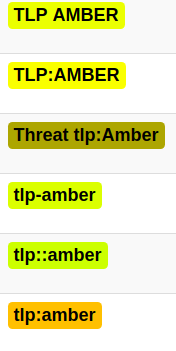
\includegraphics[scale=0.45]{screenshots/creativity.png}
    \end{center}
    \begin{lstlisting}[language=javascript,firstnumber=1]
{
    "name": "Android malware",
    "colour": "#22681c",
    "exportable": true,
    "numerical_value": null,
}
\end{lstlisting}
\end{frame}

\begin{frame}
    \frametitle{Context layer: Taxonomies}
    Simple label standardised on common set of vocabularies
    \begin{itemize}
        \item[] \textbf{Purpose}: Enable efficent classification globally understood, easing consumption and automation.
        \item[] \textbf{Usecase}: Provide classification such as: TLP, Confidence, Source, Workflows, Event type, ...
    \end{itemize}
    \vspace{1em}
    \begin{center}
        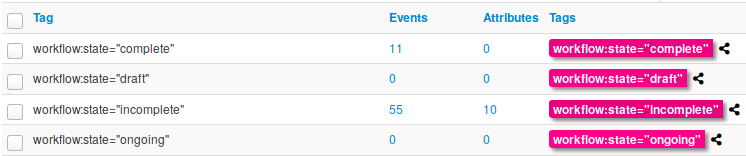
\includegraphics[width=1.0\linewidth]{taxonomy-workflow.png}
    \end{center}
\end{frame}

\begin{frame}[fragile]
    \frametitle{Context layer: Taxonomies}
    \begin{lstlisting}[language=javascript,firstnumber=1]
{
  "Taxonomy": {
    "namespace": "admiralty-scale",
    "description": "The Admiralty Scale or Ranking (also called the NATO System)...",
    "version": "6",
    "exclusive": false,
  },
  "entries": [
     {
       "tag": "admiralty-scale:information-credibility=\"1\"",
       "expanded": "Information Credibility: Confirmed by other sources",
       "numerical_value": 100,
       "exclusive_predicate": true,
     },
     ...
  ]
}
\end{lstlisting}
\end{frame}

\begin{frame}
    \frametitle{Context layer: Galaxies}
    Collections of {\bf galaxy clusters}
    \begin{center}
        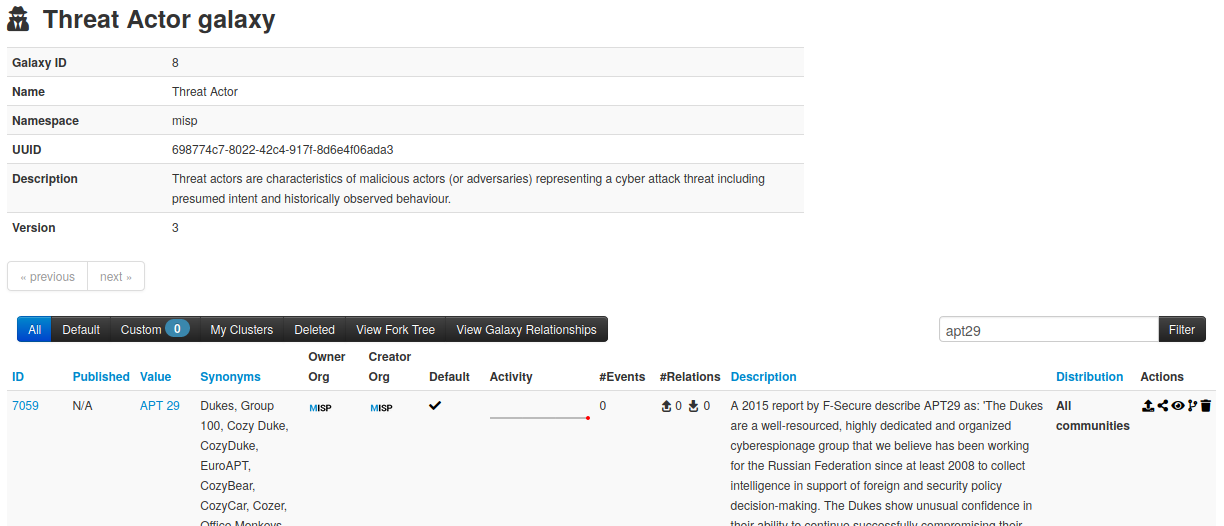
\includegraphics[width=1.0\linewidth]{screenshots/galaxy.png}
    \end{center}
\end{frame}

\begin{frame}
    \frametitle{Context layer: Galaxy clusters}
    Kownledge base items including a description, links, synonyms, meta-information and relationships
    \begin{itemize}
        \item[] \textbf{Purpose}: Enable description of complex high-level information for classification
        \item[] \textbf{Usecase}: Extensively describe elements such as threat actors, countries, technique used, ...
    \end{itemize}
    \begin{center}
        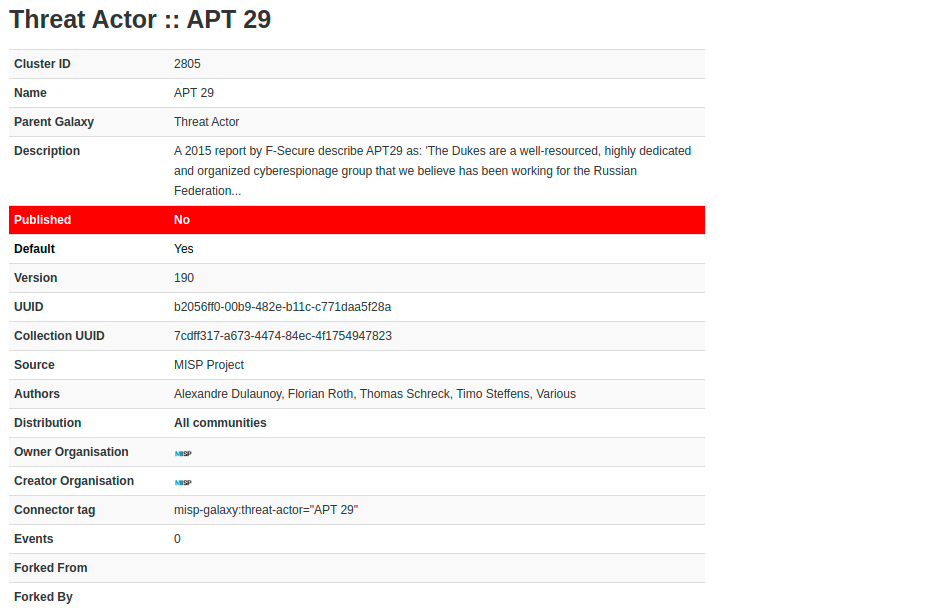
\includegraphics[width=0.65\linewidth]{screenshots/cluster-view.png}
    \end{center}
\end{frame}
\begin{frame}
    \frametitle{Context layer: Galaxy clusters}
    {\bf Galaxy cluster elements}: Tabular view
    \begin{center}
        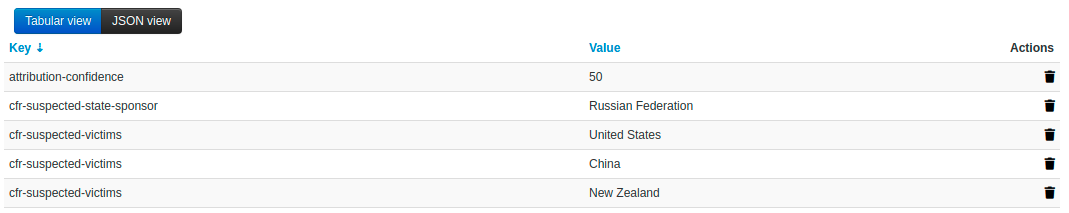
\includegraphics[width=1.0\linewidth]{screenshots/cluster-elements-tab.png}
    \end{center}
    \vspace{1em}
    {\bf Galaxy cluster elements}: JSON view
    \begin{center}
        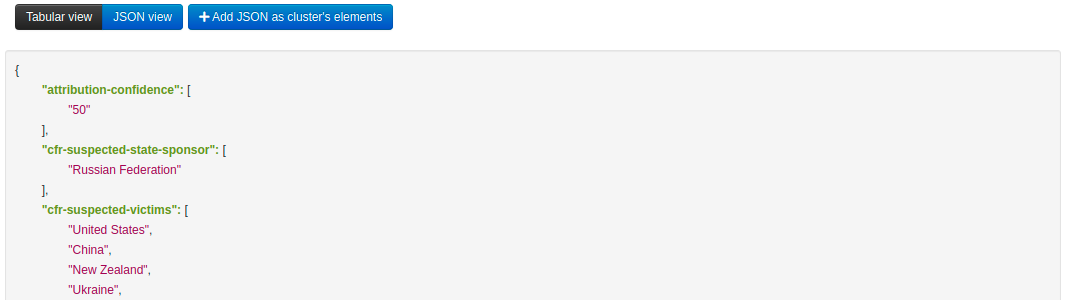
\includegraphics[width=1.0\linewidth]{screenshots/cluster-elements-json.png}
    \end{center}
\end{frame}

\begin{frame}[fragile]
    \frametitle{Context layer: Galaxy clusters}
    \begin{lstlisting}[language=javascript,firstnumber=1]
{
    "uuid": "5eda0a53-1d98-4d01-ae06-40da0a00020f",
    "type": "fellowship-characters",
    "value": "Aragorn wielding Anduril",
    "tag_name": "misp-galaxy:fellowship-characters=\"c3fe907a-6a36-4cd1-9456-dcdf35c3f907\"",
    "description": "The Aragorn character wielding Anduril",
    "source": "Middle-earth universe by J. R. R. Tolkien",
    "authors": null,
    "version": "1591347795",
    "distribution": "0",
    "sharing_group_id": null,
    "default": false,
    "extends_uuid": "5eda0117-1e14-4b0a-9e26-34aff331dc3b",
    "extends_version": "1591345431",
    "GalaxyElement": [...],
    "GalaxyClusterRelation": [...]
}
\end{lstlisting}
\end{frame}


\begin{frame}
    \frametitle{Context layer: Galaxies \& Galaxy clusters}
    \begin{itemize}
        \item MISP integrates MITRE's Adversarial Tactics, Techniques, and Common Knowledge (ATT\&CK) and similar {\bf Galaxy Matrix}
        \item MISP terminology of these matrixes: {\bf Galaxy Matrix}
    \end{itemize}
    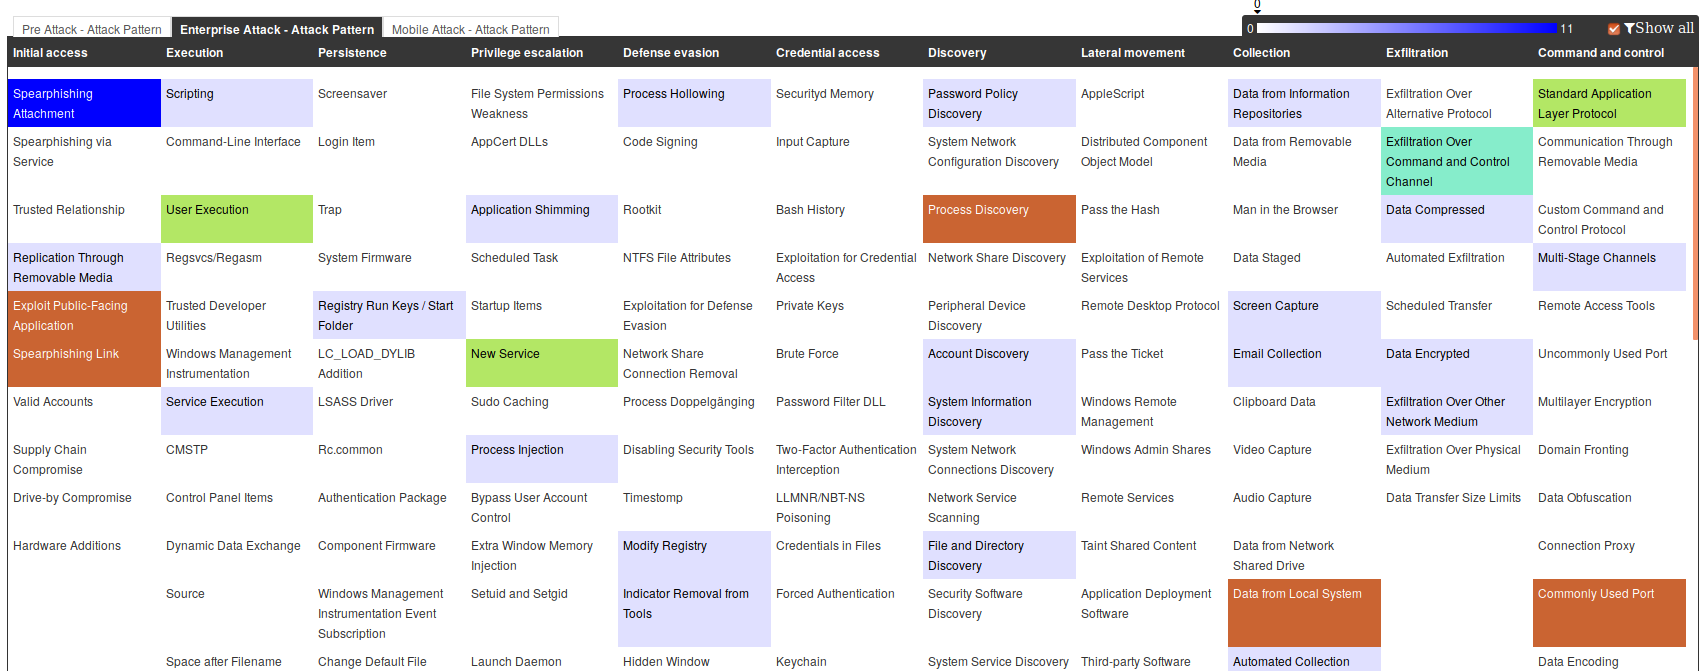
\includegraphics[scale=0.2]{screenshots/attack-screenshot.png}
\end{frame}

\begin{frame}[fragile]
        \frametitle{Galaxy JSON matrix-like}
        \begin{adjustbox}{keepaspectratio}
            %\lstset{emph={kill_chain_order},emphstyle=\textbf}
            \begin{lstlisting}[language=javascript,firstnumber=1,escapechar=@]
{
  "description": "Universal Development and Security Guidelines as Applicable to Election Technology.",
  "icon": "map",
  @\textbf{\color{red}"kill\_chain\_order": \{}@             @\textbf{\color{black}\textbackslash\textbackslash Tab in the matrix}@
      @\textbf{\color{red}"example-of-threats": [}@       @\textbf{\color{black}\textbackslash\textbackslash Column in the matrix}@
      @\textbf{\color{red}"setup | party/candidate-registration",}@
      @\textbf{\color{red}"setup | electoral-rolls",}@
      @\textbf{\color{red}"campaign | campaign-IT",}@
      @\textbf{\color{red}"all-phases | governement-IT",}@
      @\textbf{\color{red}"voting | election-technology",}@
      @\textbf{\color{red}"campaign/public-communication | media/press"}@
    @\textbf{\color{red}]}@
  @\textbf{\color{red}\},}@
  "name": "Election guidelines",
  "namespace": "misp",
  "type": "guidelines",
  "uuid": "c1dc03b2-89b3-42a5-9d41-782ef726435a",
  "version": 1
}
        \end{lstlisting}
        \end{adjustbox}
\end{frame}

\begin{frame}[fragile]
        \frametitle{Cluster JSON matrix-like}
        \begin{adjustbox}{keepaspectratio}
            \begin{lstlisting}[language=javascript,firstnumber=1,escapechar=@]
{
      "description": "DoS or overload of party/campaign registration, causing them to miss the deadline",
      "meta": {
        "date": "March 2018.",
         @\textbf{\color{red}"kill\_chain": [}@ @\textbf{\color{black}\textbackslash\textbackslash Define in which column the cluster should be placed}@
           @\textbf{\color{red}  "example-of-threats:setup | party/candidate-registration"}@
         @\textbf{\color{red}],}@
        "refs": [
          "https://www.ria.ee/sites/default/files/content-editors/kuberturve/cyber_security_of_election_technology.pdf"
        ]
      },
      "uuid": "154c6186-a007-4460-a029-ea23163448fe",
      "value": "DoS or overload of party/campaign registration, causing them to miss the deadline"
}
        \end{lstlisting}
        \end{adjustbox}
\end{frame}


\begin{frame}[fragile]
        \frametitle{Expressing relation between clusters}
        \begin{itemize}
                \item Cluster can be related to one or more clusters using default relationships from MISP objects and a list of tags to classify the relation.
        \end{itemize}

        \begin{lstlisting}[language=javascript,firstnumber=1]
        "related": [
        {
          "dest-uuid": "5ce5392a-3a6c-4e07-9df3-9b6a9159ac45",
          "tags": [
            "estimative-language:likelihood-probability=\"likely\""
          ],
          "type": "similar"
        }
      ],
      "uuid": "0ca45163-e223-4167-b1af-f088ed14a93d",
      "value": "Putter Panda"
        \end{lstlisting}
\end{frame}


\begin{frame}
    \frametitle{Acknowledgements}
    \begin{itemize}
        \item Supported by the grant \texttt{2018-LU-IA-0148}
    \end{itemize}
    \begin{center}
        
\includegraphics[scale=0.7]{en_cef.png}
    \end{center}
\end{frame}
